\chapter{Antecedents of Modern Urban Rent Theory} \label{chapter-rent}

% #NEED TO ADD THAT THIS PAPER IS MODERN URBAN RENT THEORY. AND WHAT THAT MEANS, HOW IT RELATES TO DISTRIBUTION 

\Gls{rent}, in economic theory, is different from but related to the common  meaning, which is roughly the amount you pay your landlord every month or a payment for using land or another facility.  For economists, the word normally means the  \gls{surplus} income produced by a scarce factor of production that is created by nature. You pay a high price for housing near the center of a city because land close to the city is scarce and having people close to where the jobs are is valuable. the two ideas overlap.
% #E NEED TO EXPLAIN THIS MORE BEFORE MOVING TO THE NEXT SENTENCE. DRAW OUT THE DEFINITION SO IT'S REALLY CLEAR.  

To make more sense of this idea, we need a theory location, production and money. 
for economists, that is a theory of distribution, and the first version was the classic al theory of rent. In this chapter, we trace the development of rent theory through the classical and neoclassical periods to provide context to our contribution to the development a modern urban rent theory. 

% #E OR MAYBE OPEN WITH THIS? OR: Economics is the study of ___. It is concerned with production (i.e. ___ and distribution (ie. ___) 

There are two dominant theories of \gls{distribution} in economics. The first and oldest is based on the classical concept of rent as explained  by David Ricardo \cite{ricardoEssayInfluenceLow1815}, in which owners of land are able to extract a value beyond what they contribute based on their ownership of a scarce resource. 
The second is the marginalist approach, developed by Clark and others, in which workers and other factors  in competitive markets receive the \gls{marginal value-product} of their contribution to production. The two theories coexist in modern economics.
% #E SORRY, IS THIS CHAPTER ABOUT RENT OR THEORIES OF DISTRIUTION??? MAYBE THIS STUFF ABOUT DISTRIBUTION BELONGS EARLIAR? 

Both theories developed in response to the specific social and economic conditions of the periods in which they emerged. Both attempt to explain where the output of society ends up within society. They are, at their heart, stories of who  can or does claim what share of production.  Classical rent theory  emphasized the distribution of the social surplus, the part of production  over and above what was needed to reproduce society. Initially this included only land rents, but was extended to the distribution of profit profits.  The distribution of these surplus incomes are not explained by the neoclassical theory, although profits and rents form a substantial part of national income (20–25 percent)\footnote{Schmitt, Hans Otto , Pen, Jan , Boulding, Kenneth E. and Kleinsorge, Paul Lincoln. "distribution theory". Encyclopedia Britannica, Invalid Date, https://www.britannica.com/topic/distribution-theory. Accessed 22 February 2023.} in the world the neoclassical model describes. In this thesis we identify classical rents intn the urban systems and examine their distribution.. 
% #E FIRSTNAME Ricardo was a INSERT NATIONALITY classical economist  in the WHICH Century. 


 Land produces a surplus of income. Good land produces more market value for the same cost as the poorest land in production. The poorest land in production  just justifies the cost of production but generates no surplus for its owner. more fertile land  generates more than the annual costs faced by a landowner. The difference in earning between the poorest land in ptoduction and a more fertile or better locateed field is is the quantity that economists call rent. 
 
 Landowners would generally prefer not to till the soil or bundle sheaves with their own hands, so they would `rent out' their land. The level of rent charged might not be exactly the economic rent, but in a labour surplus economy landlords would naturally have a great deal of bargaining power, and rents they charge their tenant farmers would tend to be close the value of the surplus. Rent as a price and economic rent would be practically the same.,


 As the economy shifted  moved from overwhelmingly  agricultural into the industrialization of the3 18$^th$  and 19$^th$ century economists shifte their focus from who got the rents to who got the  profits. Rent theory was eclipsed by an approach that focused on the markets for the inputs used in industrial production.  Late in the 20$^th$ century the focus has shifted to economics of  knowledge, human capital, and how cities generate wealth. The changes have resulted in changing social relations. The influence of landowners declined and the pores of  industrial capitalists in creased. More recently the the owners of industrial capital have been eclipsed  by financial capital and, to some extent, by the owners or creators of certain information technologies.


%We use the Cobb-Douglas function %, which is used to cross this entire range of literature to illustrate each link and to show how our model is directly connected with this broad collection of linked theories. 
%The Cobb-Douglas function is a production function, expressing the output produced, in terms of inputs such as labour and capital.
%Our model connects to the results in this chapter at four points:



\section{Classical theories of production and distribution and class}

The Classical theory of rent was formalized \cite{ricardoEssayInfluenceLow1815}by Ricardo in the context of a primarily agricultural economic system during increasing globalization of trade and  the early stages of the industrial revolution in Northern Europe.\footnote{The Industrial Revolution is usually described as beginning around 1760 and having significantly transformed society by about 1820–1840.}  This resulted in an increase in overall wealth while in many cases the living condition of the poor declined.  In this period, the study of political Economy was emerging as a subject of study focused on understanding trade, wealth, relationships between countries. Prior to this, international relationships centred of studies of the military, but as colonization changed the relationship between countries and trade became central, the study of political economy became more significant. 

 The early classical economists argued that all wealth came from the land and that  the tradesmen, professionals, clergy, and aristocrats were all nonproductive.\footnote{The Physiocrats, a school of economists in 18th-century France believed that land is the source of all wealth  and that government policy should not interfere with the operation of natural economic laws. They were the first to see labor as the sole source of value. However,  only agricultural labor created this value in the products of society.} In the classical tradition, rent is the value landowners claimed for the use of their land. Ricardo defines rent strictly in this way, saying ``By rent I always mean the remuneration given to the landlord for the use of the original power of the land.''\cite{ricardoEssayInfluenceLow1815} The core social question that Ricardo addressed in his theory of rent was, who gets the surplus generated by the land. This was an approach to understanding the distribution of wealth and explaining the inequality the economists were seeing. For Ricardo it provided insight into whether Britain should open its doors to corn from the colonies.\footnote{This was the debate over the Corn Laws (1794-1846), a set duties on grain imports into Britain to protect British agriculture from outside competition. In Britain, ``corn'' was the generic name for cereal crops. The full title of Ricardo's essay was was \textit{An Essay on the Influence of a low Price of Corn on the Profits of Stock, showing the Inexpediency of Restrictions on Importation: With Remarks on Mr Malthus' Two Last Publications: "An Inquiry into the Nature and Progress of Rent," and "The Grounds of an Opinion on the Policy of restricting the Importation of Foreign Corn"}.}
His model  explained the distribution of the product of the earth among the “three classes of the community” which is to say, to the owners of land, labour, and capital. 

In colloquial contexts, the term \gls{class} is often used informally as if it refers straightforwardly to people who have different levels of wealth, but when economists talk about classes, they mean something slightly different. Economic classes are functionally defined  by how they participate in production. Owners of labour participate by supplying their labour, for which they are paid a wage. Landowners own the land and receive rents for the use of their land in production. Owners of capital provide funds for starting and operating businesses, for which they receive profits.  Ricardo offered a lucid description of  how the socially produced surplus was distributed amongst these classes. %It's because the surplus is differently distributed that different have different wealth levels. 

 %This is what Ricardo developed the concept of rent to explain.  
 % \Gls{class} structure, or how different classes participate in production changes over time as modes of production change. When Ricardo was writing, the economy was still largely reflected feudal social relations in that most land ownership originated in feudal military power. %Even the land of the nobility was divided up into smaller parcels run by knights or vassals. Both of these groups traded military support for land in the local manors. As higher ranking people, knights often presided over an entire manor, while vassals presided only over the land needed to support their families.
 %  (IE DESCRIBE role of labour land, capital under feudalism and how this was changing in that period.) 
 
% The evolution of the mode of production has continued, with human capital rather than land or industrial capital increasing the source of the social surplus. The concept of rent is specifically relate to surplus and enabled Ricardo to first talk about how s is key to distribution within the economy, amongst classes.  Ricardo essentially developed his concept of Rent to explain the dynamics of distribution between classes. 


% #E i LIKE THIS STUFF ABOUT THE PHYSIOCRTAIC SCHOOL. yOU IGHT MORE DIRECTLY FRAME IT IN THE CONTEXT OF A BROADER QUESTION OF VALUE, ROLE IN PRODUCTION AND DISTRIBUTION OF SURPLUS. 
% going back to the Physiocrates. 
% The physiocratic school of economics was the first to see labor as the sole source of value but, for the physiocrats, in the context of the prevalent European rural society of the time, only agricultural labor created a surplus. % actually? % detail for it was ag economy This was the theory? also the french enginneers- detail for start of math/calc-..
%The canonical reference for only agricultural labour mattering? For the definition of rent?

% For Ricardo, and for the classical economics in general, land rent, is a kind of surplus value, that is an amount available after the costs of production have been paid, the term rent came to be used interchangeably with this more general concept in much of the classical work on rent.
% %and the term rent has been used in a more general sense to other kinds of surplus value, as well as land rents 
% #E Surplus value is essentially profit. Its the value beyond the cost. SHORT CLASSICAL EXAMPLE. Or, in a modern example, professional sports players' income, above the opportunity cost they could get working at another position, is rent they capture for their skill. 
% #E COULD ADD HERE IF YOU HAVEN'T ELSEWHERE... MAYBE ADD:
(It's easy enough to see how this concept would evolve into the two different usages of the term rent. Because it is the profit for the land, which is related to payments for the land. At the time, the feudal ownership structures meant that the value of the land was structured differently. Tenants did not pay to occupy the land the way that people and businesses do today. Rather the value of owning land was reflected in the distribution from production. The term later split to reflect both the way land is currently valued (i.e rent payments to occupy) and the surplus value that was how land was valued in the period of clssical econmics with it's feadul structures. Rent became payment to landlord because under feudalism, the surplus went to the landlords. Thenn the term diverged into the two distinct meanings used colloquially and in a technical context by Economists ) 

The classical idea of rent and rent % #E RENT AND RENT??? .... can be illustrated with the story of a carter % call it a distributor/worker?
who picks up vegetables at the farm gate, transports them into town, and sells them to a storekeeper. %He pays the farmer at one end of the trip and is paid at the other. 
% #E NEED TO CLARIFY WHO OWN WHAT AND HOW LAND IS UCCUPIED UNDER THE ECONOMIC STRUCTURES OF FEUDALISM,
For simplicity, assume all farmers have the same cost of production, and the carters pay the farmer the farm gate price at the farm and receive the merchant price in town. 

\begin{figure}
    \begin{center}
     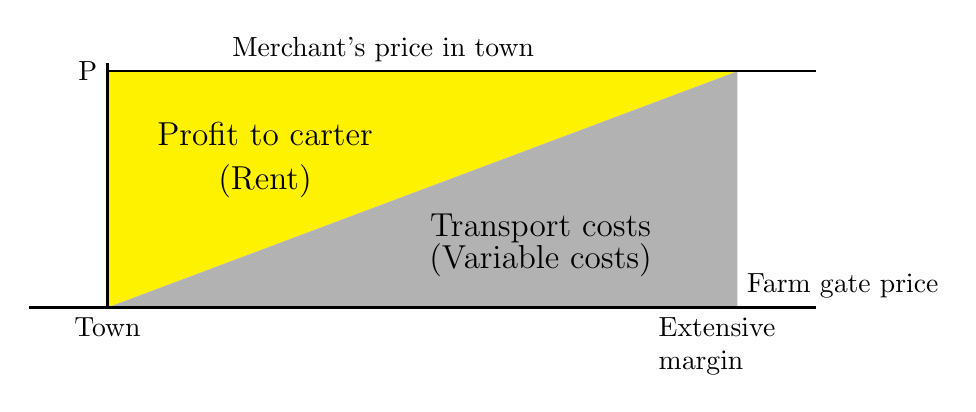
\begin{tikzpicture}[domain=0:2]
%\draw[thick,color=gray,step=.5cm, dashed] (-0.5,-.5) grid (3,3);
%\draw[line width=.01, green ] (0,0) -- (10,0) node[right  ] {Distance};
\node at (1,0) [below] {Town};
\fill[yellow]  (1,0) --(9,3)--(1,3) --cycle;
\fill[gray!60] (9,3) --(1,0)--(9,0) --cycle;

\draw[thick ] (1,3)node[left]{P}  -- (10,3);\node at (4.5,3)[above ] {Merchant's price in town} ;
\draw[thick ] (0,0)  -- (10,0); 

%\draw[thick,color=red] (1.5,0) -- (1.5,1) node[below right] {Fixed cost} -- (1.5,1.5) --(10,3.25)node[above left] {total cost};
\draw[thick] (1,0) -- (1,3.1) ;
\node[below,text width=2cm]at (9,0) {Extensive margin};
%\draw[ultra thick, blue,<-> ] (3,1.8) -- (3,2.5)node[left] {annual rent at a} -- (3,3) ; 
\node at (9,0)[above right] {Farm gate price};
\node  at (6.5,1){\large Transport costs};
\node  at (6.5,.6){\large (Variable costs)};
\node  at (3.,2.2){\large Profit to carter};
\node  at (3.,1.6){\large (Rent)};
\end{tikzpicture} 
    \caption{Transport costs, the yellow area, take a share of the profit for vegetables sold in the town}
    \label{fig-rent-ricardo}
    \end{center}
\end{figure}

In the figure \ref{fig-rent-ricardo}, total transport costs are shown as the yellow area. The area below the yellow triangle is profit for the carter. The carter makes a `profit' on the trip to the farm nearest to town, but at a certain distance, the transport costs will eat up all the profit on the trip. That is as far as the carter will go\footnote{Note the similarity with Alonzo's urban model, illustrated in Fig \ref{fig-rent-alonzo}.}
Ricardo termed this point the `extensive margin', the point at which there is no value for farming for the town. It is the limit for this use, and the profit there is zero. If the price goes up, the extensive margin moves out, and more land comes into production.

The land rent declines with distance from the town,\footnote{% #E ADD?? This graph is simplified to illustrate the concept.
It also declines for less fertile land, where there is a higher cost of production.} At the extensive margin the land rent falls to zero. Even fertile land beyond the extensive margin will not be farmed because the product cannot be transported to market at a profit.\footnote{This simple example assumes that the land is uniformly productive and that there is only one product that can be marketed. Johann Heinrich von Th\"unen, in The Isolated state (Der isolierte Staat (1826)), provide a more complex analysis based on the same principles.} Transportation costs and the price of produce in town determine the size of the  rent triangle and therefore the amount of rent captured by the land-owning class.\footnote{The debate about the  `Corn Laws" that Ricardo  was engaged in was about whether Britain would allow wheat form Canada and Australia to enter, reducing the price of wheat and therefore reducing the income and influence of the land-owning class.} 

Together these two triangles/areas represent the ``produce of the earth'', but only the lower triangle is net income\footnote{ Termed the `\textit{produit net}' by the Physiocrats}. In modern supply and demand analysis it would be recognized as `producer surplus', the difference between what a producer gets for a good and what they would be willing to accept.

In Ricardo's case: the land owner delivers the grain to market and receives the merchant price. The profit is what the landowner could claim for the privilege of using the land %The profit now accrues to the landowner, and we call it land rent. For Ricardo, it was obvious that the land-owning class captured the land rent.
\footnote{In the modern economy, agricultural land rents may be captured by corporations,  either by owning the land or by controlling the supply chain.}  Landlord income is a locational land rent that exists because of the land's proximity to the market. 
 

%\subsection{A more explicit treatment}
as Saunders says in 1902, ``Of the concrete forms of income that have usually been classed as surplus, the rent of land was the earliest to be defined; and so prominent a position has been given to it that the terms "rent" and "surplus" have come to be used interchangeably.'' \footnote{Rent in Modern Economic Theory: An Essay in Distribution Author(s): Alvin Saunders Johnson, Publications of the American Economic Association, Nov., 1902, 3rd Series, Vol. 3, No. 4 (Nov., 1902), pp. 1-129}. 

Ricardo expounded his theory of land rent % #E AD::  prior to the emergence of  WHAT?? Mathematical ____ . While he did not write down a formal production function as later neoclassical theorists would, modern neoclassical production theory can be seen as having one of its origins in his work on classical economic theory. % #E Where does this go ... put with explanation of how neo-classicists were influences by Ricardo

While he did not write down a formal production function as later neoclassical theorists would, his theory can be put in the notation neo-classicists used /developed. In modern notation, Ricardo's model can be written: 

\begin{equation} 
Y=F(K,L,N).
\label{eqn-production-ricardo}
\end{equation} 

where $K$ is capital, $L$ is labour and $N$  is the natural resource land.\footnote{This makes it a three factor model of production (cite us/lit) In principle any number of factors can be included.}  
Ricardo does not specify a functional form, but, %like mathematical neoclassical economists, 
he does assume diminishing returns to all factors. The landlord  receives the surplus generated by the land and the rest of the value of production goes to labour and to any capital employed in improving the land. 

The value of the land is the present discounted value of the surplus it generates, that is what it would be worth paying now, to capture the future rents from that land.


\subsection{Marx}


%Ricardo, agreeing with Malthus, essentially assumes that the wage is  just sufficient to reproduce the labouring class.\footnote{``In the natural advance of society, the wages of labour will have a tendency to fall, as far as they are regulated by supply and demand; for the supply of labourers will continue to increase at the same rate, while the demand for them will increase at a slower rate.''} He then explains the distribution of the fruits of labour on the land among the main classes of the economy.
%#E ADD CONTEXT like:
By the time Karl Marx was active in TIME PERIOD, European economies were largely structured around manufacturing. 

 Marx shifted attention % #E MORE ACCURATE TO SAY HE was exploring this because it was what he saw than shifted attention.
 In the manufacturing economy, the owners contribute the machinery, buildings, and even working capital to fund the workers until the product can be sold. % #E FLESH OUT THIS DESCRIPTION OF THE KEY FEATURES OF TEH MANUFACTURING ECONMY. ALOS SPECIFCAL DEFINE CAPITAL CAN WHY IT MATTERS
 %This contribution must be accumulated from their profits in the preceding cycle of production,  and has to be reinvested once the revenues of the current round have come in and the bills have been paid. Marx actually describes a circuit of capital from its form as money to its form as physical capital. 
As in Ricardo, however, labour is in surplus and capital is scarce. As in Ricardo the scarce factor owned by a special class - now the capitalists, is able to appropriate the is able to capture the surplus value. %Like Ricardo,  Marx saw the appropriation of surplus as without moral justification. 

Marx pointed to a new dynamic in capitalist systems - that productive capital is not fixed as land is, but  expands as surplus is reinvested. % #E EXPLAIN WHAT THIS MEANSAND WHY IT MATTERS TO DISTRIBUTION. HOW IS IT DIIFFERENT OR SIMLAR TO WHAT WAS HAPPENING UNDER FEUDALISM? 
%He famously suggested that the expansion will eventually outrun the expansion of demand and the rate of return will fall, leaving capitalists unwilling to invest. % and creating a crisis. 

Marx gives the statement of the dynamic quality of the surplus
- work linking urban rents to the dynamic quality of the surplus in the urban system is in that tradition 
- how does the generative surplus gets distributed, its dynamics/the dynamics of the surplus. % #E SEEMS TO BE A LOT MISSING HERE?

% #E i FEEL LIKE IT WOULD BE USEFUL TO DESCRIBE THE CLASS BREAKDOWN IN MARX AS IT RELATES TO HOW THE DIFFERENT ROLES FIT INTO PRODUCTION. aLSO. WHAT HAPPENED TO THE IDEA OF LAND RENT IN THIS PERIOD AND IN MARX'S WORK SPECIFICALLY? dID HE IGNORE IT? EVEN IF HE DIDN'T USE THE CONCEPT, EXPLAIN HOW IT WOULD RELATE OR FIT (OR NOT FIT) INTO THIS CONCEPT)
 
\subsection{Henry George} 


  Henry George, an influential American political economist IN WHAT PERIOD??? ,\footnote{Progress and Poverty: An Inquiry into the Cause of Industrial Depressions and of Increase of Want with Increase of Wealth: The Remedy (1879) book by social theorist and economist Henry George.}  returned to land rent with a new insight based on the emergence of the capitalist city: ``With the growth of population, land grows in value, and the men who work it must pay more for the privilege.'' For George the owners of urban land extract surplus in exactly the same way that owners of agricultural land in Ricardo's analysis. % #E MAYBE ADD: Like Marx, George predicted that the system would lead to a crisis, but
  Where Marx saw the extravagant productivity of capital as the source of capitalist crises, George saw the extraction of wealth by land speculators as the mechanism that would bring on crises.
  % #E WHAT DID HE MEAN BY CRISIS? HOW DID HE COME TO BE CONCERNED ABOUT THIS? ALSO SINCE YOU ARE COMPARING WITH MARX's PREDICTIONS ABOUT CRISIS YOU NEED TO EXPLAIN MORE ABOUT MARX'S IDEAS OF CRISIS ABOVE
  % #E Somewhere in HERE YOU MAY WANTED TO EXPLAIN SOCIALISM VS MARXISM... GEORGE IS SOCIALIST? MARX?? PUTTING IN THE CONTEXT OF HOW THOSE TRADITIONS WERE EMERGING MIGHT BE HELPFUL... I HAD THIS NOTE ON THE PAPER DRAFT... COULDN'T FIGURE OUT WHY SINCE YOU DON'T SAY GEORGE IS A SOCIALIST. bUT YOU DO LATER WHEN YOU EXPLAIN THE SHIFTS IN jb CLARK'S THINKING. IF YOU WANT TO CONTEXTUALIZE CLARK IN TERMS OF SOCIALISM ... BEST TO MAKE SURE YOU'VE EXPLAINED THAT GEORGE IS A SOCIALIST, WHAT THAT MEANS, AND THEN, SINCE MARX IS FAMOUSLY BUT CONFUSINGLY INTERCONNECTED WITH SOCIALISM YOU SHOULD EXPLAIN HOW HIS THINK AND (SEPARATELY) THE MOVEMENT NAMED AFTER HIM FIT IN) 
  % # ADD George also presented solutions to ____ 
  
  Since land rent is not created by its owners, George argued that land rent should be seen as a social income - that it could be used to pay for all the needs of the community. The clearest statement of this view is found in Progress and Poverty when he wrote "We must make land common property." The same view was expressed by the Physiocrats who concluded  that ``ground rents'' should be the source of most or all taxes. They defined ground rent as that portion of all rent which is attributable only to the size and location of the parcel. George's analysis the `single tax' movement, which sought to shift all taxation to land  and resource rents.   

  
Even as Ricardo was writing, the industrial revolution was changing what Marx called the mode production changed. The influence of landowners declined and the owners of more liquid forms of capital became increasingly powerful. Thinkers like Marx and Engles revised and extended  class theory to account for growing power of the capitalists.  By the late nineteenth  century a new school of mathematically inclined economists focused on how competition regulated the distribution of wealth. They shifted the emphasis from ownership of the factors of production to the marginal product of the factors of production in competitive markets. It was eventually shown that the distribution under competition is, if not fair,  is at least efficient in a specific sense.\footnote{The result is known  in economics as the ``First Fundamental Theorem of Welfare Economics.'' The basic idea goes back to Adam Smith and was gradually developed  ver 70 years until Kenneth Arrow and Gérard Debreu (separately, 1951) each gave  a satisfactorily general proof in 1951. In 1986 %their 1986 paper, ``Externalities in Economies with Imperfect Information and Incomplete Markets''
Bruce Greenwald and Joseph Stiglitz showed that the fundamental welfare theorems do not hold if there are incomplete markets or imperfect information.}

  
  In 1977, Joseph Stiglitz, using Alonzo's relatively new urban model, identified the conditions in which Henry George's "single tax" is  the only tax necessary to finance public expenditures.\footnote{Arnott, Richard J.; Joseph E. Stiglitz (November 1979). "Aggregate Land Rents, Expenditure on Public Goods, and Optimal City Size" (PDF). Quarterly Journal of Economics. 93 (4): 471–500. doi:10.2307/1884466. JSTOR 1884466. S2CID 53374401 }   The logic is fairly simple: if the public good increases productivity or the attractiveness of a city, attracting more people or businesses, land rents rise, and investment in the public good should proceed until the marginal cost of the public good is equal to the increase in land rent it brings. The result is now called the `Henry George theorem.'



The classical economists agreed that rents are unearned income. They did not emphasize, as George did, that land rents arise from labour's proximity to urban population and production.\footnote{To be fair, it was not lack of understanding, that the omission reveals, but rather lack of interest in explicitly examining urban land rent from residential or even industrial purposes.}% Ricardo von Thunen, Marx, Cantillon all grasped the notion of proximity to the market as part of the source land rent. The discussions seem to not gone farther than discussions of diffeerential and rents, however.  I just am not aware of them explicitly examining urban land rent for residential or even industrial purposes. 

%The need to be near a market or prodduction center is easily seen by considering a population at the carrying capacity of the land with individuals supporting themselves using purely local resources. There can be no land rent in this case. If a city rises that must be supplied from those still on the land, land close enough to the city will generate land rent. The value of the land is created by proximity to the city.



%  no separate and comprehensive data are provided on the amounts of land rents and subsoil rents charged and earned, because they are not officially regarded as part of value-added, and consequently are not included in the calculation of GDP (except for the value of productive lease contracts)     https://en.wikipedia.org/wiki/Differential_and_absolute_ground_rent#Rent_in_macro-economics    \href{https://en.wikipedia.org/wiki/Differential_and_absolute_ground_rent#Rent_in_macro-economics}{Wikipediat article on differential rent}

Stiglitz % maybe ADD: takes this a step further by linking...
is linking the capture of urban rents to productivity.

  \subsection{John Bates Clark and neoclassical distribution theory}
  % # NEED SOME MORE CONTEXT HERE. maybe atart by setting up the PERIOD WE ARE NOW MOVING INTO AND WHAT HAS SHIFTED IN THE ECONOMIC STRUCTURE? 
  
  Classical theories of distribution showed that ownership of a scarce and non-produced factor, land, was the  basis of rent extraction by the class of landowners. Profits were a bit puzzling in this context - Capital also earns its return from scarcity. % #E i DON'T UNDERSTAND WHY PROFITS ARE PUZZLING? WHATS THE QUESTION? eXPLAIN MORE.
  Marshall % #E WHO IS THIS? DATES? LOCATION?
   pointed out, however, that scarcity profits (i.e., rent) would normally be competed away  as entrepreneurs entered the market in pursuit of those `excess' profits. He used the term `pseudo-rents' for these unearned but temporary incomes.\footnote{Alvin Saunders Johnson. Rent in Modern Economic Theory: An Essay in Distribution. AEA 3rd Series, Vol. 3, No. 4 (Nov., 1902), pp. 1-129 (129 pages)}

 John Bates Clark was one of the pioneers of marginalism and the neoclassical theory of  distribution.  The marginalist approach emphasized the rational decisions of economic agents in allocating their resources would lead them to allocate resources according to the value of the marginal product % #E DEFINE MARGINAL PRODUCT
 of the resource in production.  
 Initially a socialist like George, % #E YOU NEED TO HAVE SAID ABOVE GEORGE IS A SOCIALIST OR CUT THIS. 
 by 1986 he was praising the dynamical process of competition partly in opposition to the single tax movement George had initiated.  His (1891) ``Distribution as Determined by a Law of Rent,'' argued that, given  competition and homogeneous factors of production labor and capital, the division of the social product will be according to the productivity of the last (or marginal) physical input of units of labor and capital.\footnote{Responding to the "indictment that hangs over society" that it involves "exploiting labor," Clark wrote:

    It is the purpose of this work (his 1899 'Distribution of Wealth) to show that the distribution of the income of society is controlled by a natural law, and that this law, if it worked without friction, would give to every agent of production the amount of wealth which that agent creates. However wages may be adjusted by bargains freely made between individual men (i.e., without labor unions and other "market imperfections", the rates of pay that result from such transactions tend, it is here claimed, to equal that part of the product of industry which is traceable to the labor itself; and however interest (i.e., profit) may be adjusted by similarly free bargaining, it naturally tends to equal the fractional product that is separately traceable to capital.} 

 In Clark's  perfect competition,% #E I THINK YOU NEED A BIT MORE ABOUT COMPETITION AS A CONCEPT AND IT'S HISTORY. ITS PRETTY IMPORTANT. ALSO MAYBE REFERENCE ADAM SMITH ? 
 
 each factor of production—capital and labor—gets its just reward based on its contribution of  the last unit employed to a company’s profits. A more realistic description of the world is one of imperfect competition, where the division of the economic pie is based not just on the relative contributions of capital and labor to the bottom line but on their relative bargaining power. 
 
Clark's analysis of income distribution does not contradict the classical view of rents, it simply displaces the analysis to the point where a competitive equilibrium prevails, and shifts attention away from the distribution of land rents. Rents are not earned by the marginal unit of land and therefore the share to land at the margin is zero. 



\section{Neoclassical production theory}
The concept of a production function used by increasingly mathematical neoclassical economists and  rapidly developing statistical techniques  naturally led to attempts to identify the precise functional form that would describe the contributions of labour, capital, and income to output.
 
Mathematician Charles Cobb and Economist Paul Douglas came up with a specific and very convenient functional form\footnote{Cobb, C. W.; Douglas, P. H. (1928). "A Theory of Production"  American Economic Review. 18 (Supplement): 139–165. JSTOR 1811556. Retrieved 26 September 2016. The function had apparently previously been used by Knut Wicksell, Philip Wicksteed, and L\'eon Walras.} that captured much of what economists were talking about. The function is just a generalized arithmetic mean:
 
 \[Y=AK^\alpha L^\beta\]
 where $A$ is a constant scale factor, commonly called `Total Factor Productivity. This function becomes the workhorse of neoclassical growth theory in the second half  of the 20th century. Our urban model is a direct heir of those developments.

%The Cobb Douglas function has several convenient features. One is that the sum of the coefficents tells us the degree of returns to scale. If $\alpha+\beta = 1$, we have constant returns to scale,

%Another is that the coefficients of the factors, $\alpha$  and $\beta$ turn out to be the elasticities of output with respect to capital and labour respectively as well as the income share of the factor. These made it relatively easy for economists to combine national data on labour and capital stocks or income with output to test the model.

The Cobb–Douglas form was developed and almost immediately tested against statistical evidence in the USA by Cobb and Douglas between 1927–1947. It was  their widely circulated empirical work seems to have permanently associated this simple function with Cobb and Douglas for economists.

\section{Classical vs neoclassical production theory}

Ricardo's analysis of land  can be thought of as focusing only on land:

\begin{equation} 
Y=F(L,N).
\label{eqn-production-ricardo-2}
\end{equation} 
where $K$ is capital, $L$ is labour and $N$  is the natural resource  land.

Most modern neoclassical treatments of production have the same basic structure of the production function, but they simplify by omitting land and emphasized capital:
\begin{equation} 
Y=F(K,L).
\label{eqn-production}
\end{equation}  
which makes sense for a number of reasons. The economy has shifted from agriculture to industry and the4 focus of economic theory has shifted to manufacturing processes.
%Leaving land out of the model makes sense for a variety of reasons. 
Furthermore, according to the Ricardian theory, rent is a surplus above cost. It does not, therefore enter into price. Land is a fixed factor for society as a whole that is not consumed in  the process of production.  Neoclassical treatments of production focus price determination based on the cost of the last unit used, the marginal  unit of input, while rents are generated on all of the inframarginal units, those units used earlier, which are more productive. The marginal unit of land generates no rents. In neoclassical analysis, the rents disappeared from view for this reason. This difference is at the heart of the distinction between classical and neoclassical economic theory. 

%John B. Davis. Ricardo's Theory of Profit and the Third Edition of the \textit{Principles}. Journal of the History of Economic Thought, 15, Spring 1993. °1993 by the History of Economic Society.
%``Questions arise, however, when one turns to exchange between a sector paying rent and one not.'' The Principles tells us that as cultivation is extended and exchange increases, profits fall while rents increase. 

Leaving land out, however, creates a problem in  the neoclassical growth theories we will examine below. Under the assumption of perfectly competitive goods and factors markets as well as marginal productivity pricing of capital and labor, neoclassical growth requires technical change to be generated outside the model because there are no resources left to innovate if both factors of production are paid their marginal product.\footnote{This follows from Euler’s theorem: if, for a given level of technology $\bar A$ output Y is produced according to a \textbf{constant returns to scale} and twice continuously differentiable function of capital and labor $F(K, L, \bar A)$, Euler’s theorem implies that $F_K K + F_L L=Y$, where $F_i$ is the marginal product of factor $i$. Payments to  capital and labor take up the entire national product and no resources are left to finance the production of technology-improving innovations. are paid their marginal product.} 
If, however, land is reintroduced, as it must be in an urban model, there must be rents and there is therefore a surplus available for innovation.
\footnote{An alternative and common approach is to assume imperfect competition, which may be based on increasing returns to scale, in which case firms with market power may achieve a surplus. ``Although seldom modeled outside the monopolistic competition framework, market incompleteness and imperfect competition are central to the new growth theories'' (Gilles Duranton, Growth and imperfect competition on factor markets: Increasing returns and distribution, European Economic Review, 44-2, 2000, 255-280), Similarly, Sjak Smulders and Theo van de Klundert conclude that ``Growth is higher in a more concentrated market provided that market power of firms is not too high,'' (Imperfect competition, concentration and growth with firm-specific R \& D, European Economic Review, 39-1, 1995,139-160).}
%I have not followed this track down to give references.

% ALSO Imperfect Competition and Total Factor Productivity Growth  AZZEDDINE M. AZZAM, ELENA LOPEZ and RIGOBERTO A. LOPEZ. Journal of Productivity Analysis. Vol. 22, No. 3 (November, 2004), pp. 173-184 (12 pages)

%Sjak Smulders and Theo van de Klundert.Imperfect competition, concentration and growth with firm-specific R & D European Economic Review. Volume 39, Issue 1, January 1995, Pages 139-160
% Duranton, Gilles (1997) Essays on growth: imperfect competition, labour supply and local public goods. PhD thesis, London School of Economics and Political Science.  http://etheses.lse.ac.uk/1471/1/U105715.pdf

%\footntoe{Alberto Bucci.  R&D, Imperfect Competition and Growth with Human Capital Accumulation, 2003. Scottish Journal of Political Economy. https://doi.org/10.1111/1467-9485.5004004. This paper studies the long-run consequences of imperfect competition on growth and the sectoral distribution of skills within an R&D-based growth model with human capital accumulation. We find that steady-state growth is driven only by incentives to accumulate skills. In the model imperfect competition has a positive growth effect, while influencing the allocation of human capital to the different economic activities employing this factor input. Contrary to general wisdom, the share of resources invested in R&D turns out not to be monotonically increasing in the product market power and its correlation with the equilibrium output growth rate is not unambiguous.}

%NOTE URBAN COMPETITION PROVIDES INCENTIVES TO UPGRADE SKILLS!!!


% Both the Solow (1956) growth model and its Ramsey–Cass–Koopmans counterpart featuring an endogenous saving rate (Ramsey, 1928; Cass, 1965; Koopmans, 1965) but treat technical change as purely exogenous. In fact, under the assumption of perfectly competitive goods and factors markets as well as marginal productivity pricing of capital and labor, neoclassical growth requires technical change to be generated outside the model because there are no resources left to innovate if both factors of production. 

% 
% assuming that technical progress is labor augmenting (Uzawa, 1961), we can rewrite the production function as $F(K, AL$), where $AL$ is a measure of labor in efficiency units, or effective workers. Let k = K/(AL). Then, output per effective worker is y =Y/(AL)=f (k). Population grows at the constant rate n > 0 and, as we will assume throughout the whole paper, capital does not depreciate. The steady state of the Solow model solves

% $\frac{f(k_{ss}}{k_{ss}} = \frac{n+g_A}{s}kss s$

% Journal of Economic Surveys (2017) Vol. 31, No. 5, pp. 1272–1303 \c ECONOMIC THEORIES 1275


Classical rent re-appears in neoclassical theory as `economic rent' (``a money payment made for a factor of production that is over and above the minimum payment to keep it in its present use,'')  as quasi-or pseudo-rents (non-equilibrium rents that will be competed away in a competitive equilibrium according to Marshall.\footnote{see Lewis Cecil 4 Rent Under the Assumption of Exhaustibility, Quarterly Journal of Economics, May, 1914, Vol. 28, No. 3 (May, 1914), pp. 466-489}),  as consumer  and producer surplus in supply and demand analysis,  as rent profiles or Pseudo-rent curves in urban theory, as a major concern on resource economics, and the theory of rent-seeking. Economic rent is a surplus insofar as its payment is not necessary to ensure a supply of a particular factor of production. 


% HOUSING RENT IN THE NATIONAL ACCOUNTS
%   Owner-occupied housing is included in Peersonal Consumption Expenditure because the National Income and Producgt Accounts (NIPAs) treat the owner-occupant as if it were a rental business, or in other words, a landlord renting to him or herself. That is, BEA imputes a value for the services of owner-occupied housing (space rent) based on the rents charged for similar tenant-occupied housing, and this value is included in GDP as part of personal consumption expenditures. This imputation is necessary in order for GDP to be invariant when housing units shift between tenant occupancy and owner occupancy.


%Ricardo  clearly understood and used the concept of diminishing marginal product. This shows in his use of the terms ``extensive margin'' and ``intensive margin'' to explain the income of the landowner. He focussed on the difference between the cost of production on a unit of land and the revenue generated. The landlord would rent out all the land which generated at least enough to pay all the costs. Anything in excess of the costs could be charged as land rent to a tenant farmer.



%Clearly in his model there are two basic productive factors, land and labour. The landlord  receives the surplus generated by the land and the rest of the value of production goes to labour. 
Recent urban models, on the other hand, tend to ignore the production process and consider the locational implications of land and transportation costs on the location of people. Wealth distribution is often ignored. 




\subsection{TEMP/MOVE - marginalist distribution}
% MARGINALIST DISTRIBUTION
% we've been paying some people less than the market wage so our profits our higher. this is what it would be if we paid everybody

% FOOTNOTE - RELATIONSHIP with marginalist distribution story ******** TODO Does the marginalist approach assume they are not exploited? Is it an experiment in examining the case where production is non-exploitative? 
% In a sense if labour gets the marginal value of their product, are they exploited. It's a matter of interpretation.  -It has an attraction 
%Clark tried to make an ethic of this. if everyone is being paid the marginal product of their labour. We know that's an efficient outcome. If it's efficient, is it also fair
%Is it possible someone's taking out an extra large fair. Yes. Not fair for simple classical reason that labour has been exploited in the past and that the current owner ship is a result of exploitation. The ownership of land introduces a kind of exploitation-- clearly exploitation if you claim that. 
%Lot's of marxists didn't like Henry George making it a locational question, they wanted to keep it located in the factory.
% You could - well what value did they create -- in line with those other-- could interpret.. 
%What is the average value, because every worker is not just marginal, they're also average/identical. What is the value created by the whole of the workforce. Should they be paid the marginal value or the average value of their work.
%
%The avg value -- declining.. 
%The demand for labour is declining--  
%Every infra marginal worker has been paid less than the avg contribution 
%Every infra marginal workers should - 
%every marginal worker should get the average wage.. that's fair.
%
%Get to the margin - that's what you pay.. that's what the next worker is worth to the firm. .. 5th' worker is paid more than the 10th. should it be averaged out and paid to all workers? paid to worker, or should the difference between top and the marginal goes to the firm- -- that's profit.. pay everyone the marginal value and keep the rest as profit.. 
%Effective labour has a higher marginal product.. - even higher - higher for the firm.. - but they don't have to pay the workers that... firms only have to pay enough to get their marginal individual cost down to the wage. The problem there is if they're making more profit they want to expand the workforce, but that wage only supports a certain size of city -- they've got off raise the wage a bit.. so they face an upward sloping supply curve for labour=-- that's why you know there's an equilibrium.. declining product and upward sloping supply so they cross.
%
%(all the profit you earn on the way could be redistributed)

